\documentclass{iuthesis}

\usepackage[utf8]{inputenc}
\usepackage{bigstrut}
\usepackage{cite}
\usepackage{graphicx}
\usepackage{latexsym}
\usepackage{lingmacros}
\usepackage{rotating}
\usepackage{setspace}
\usepackage{textcomp}
\usepackage{url}

\title{Cross-lingual Word Sense Disambiguation for Low-Resource Hybrid Machine
Translation}

\author{Alexander James Rudnick}

\advisor{Michael E. Gasser}
\secondreader{Sandra C. Kübler}
\thirdreader{Markus Dickinson}
\fourthreader{David J. Crandall}
\fifthreader{John S. DeNero}
\departmentname{School}
\department{Informatics and Computing}
\copyrightyear{2014}
\submitdate{September 2014}
\acceptdate{09/24/2014}

% for use with the iuthesis-alt.cls
% \parskip=6pt
% \parindent=0pt
% \normalparindent=0pt

% Helpful for TODO and TBD in the output of the file (in red)
\newcommand{\TBD}[0]{{\color{red}TBD}}
\newcommand{\TODO}[1]{\noindent{\color{red} TODO: #1}\\}

\makeindex

\begin{document}
\frontmatter

% somewhere in here is also the dedication, which is not the same as the
% acknowledgements, but sort of similar.
\begin{acknowledgements}
TBD
\end{acknowledgements}

\begin{abstract}
Abstract Here
\end{abstract}

\maketitle
\signaturepage
\copyrightpage
\makededication
\makeabstract
\tableofcontents

\mainmatter

\section{Overview}
In this dissertation, I will investigate techniques for building a hybrid
machine translation (HMT) system for a language pair with relatively modest
resources.
I propose that cross-lingual word sense disambiguation (CL-WSD) is a feasible
and practical means for lexical selection in this setting, and will work to
demonstrate this by using it to construct a HMT system for Spanish and Guarani,
the co-official languages of Paraguay.
Along the way, I will develop new CL-WSD approaches, including the use of
multilingual evidence and sequence-labeling techniques, and also crowdsourcing
approaches for collecting larger corpora for disadvantaged languages.

Lexical ambiguity presents a serious challenge for rule-based machine
translation (RBMT) systems, since many words will have multiple possible
translations in the target language. Moreover, several translations of a given
word may all be syntactically valid in context, but have significantly
different meanings. Even when choosing among near-synonyms, we would like to
respect the selectional preferences of the target language so as to produce
natural-sounding output text.

Writing lexical selection rules by hand is tedious and error-prone; bilingual
informants, if available, may not be able to enumerate the contexts in which
they would choose one alternative over another. Thus we would like to learn
from corpora when possible. However, for most language pairs, suitably large
sentence-aligned bitext corpora are not available, so creating and deploying a
translation system based on machine learning techniques will require collecting
a larger corpus.

The major contributions of this work will be new approaches for: CL-WSD,
integrating CL-WSD into RBMT systems, and crowdsourcing bilingual data
collection to a relatively small though engaged population.
Additionally, on a practical level we will develop: a suite of reusable
open-source software; a practical MT system for the Spanish-Guarani language
pair; a website where language learners and activists can help build large
bilingual corpora; and a freely available corpus of Spanish-Guarani bitext.

In this work I will focus on Spanish and Guarani, the co-official languages of
Paraguay. I will describe novel approaches to CL-WSD, including using evidence
from multilingual sources and sequence labeling techniques.  I will also
investigate the collection of a larger bilingual corpus through crowdsourcing
and the integration of the disambiguation techniques into a rule-based
translation engine, producing a hybrid rule-based/statistical translation
system. Along the way, I will also work on integrating our CL-WSD techniques
into other rule-based MT engines.

\subsection{Thesis statement}
Cross-lingual word sense disambiguation (CL-WSD) is a feasible and practical
means for lexical selection in a hybrid machine translation system for a
language pair with relatively modest resources.

\subsection{Questions to address}
\begin{enumerate}
\item Which CL-WSD techniques are useful for our purposes?
\item Which kinds of MT systems can benefit from CL-WSD?
\item How can we collect bigger corpora to train our system?
\end{enumerate}


\section{Cross-lingual Word Sense Disambiguation}

Cross-lingual word sense disambiguation (CL-WSD) is the task of labeling tokens
in the context of an input sentence ... ; this has a clear application to
machine translation, in that  ...

Treating lexical selection as a word-sense disambiguation problem in which the
sense inventory for each source-language word is its set of possible
translations is often called cross-lingual WSD (CL-WSD).

In a cross-language word-sense disambiguation (CL-WSD) task, given an
instance of an ambiguous word used in a context, we want to predict the
appropriate translation of that word into the target language. This setting for
WSD has an immediate application in machine translation, since many words have
multiple possible translations.

There have been shared tasks on CL-WSD at recent SemEval workshops; the most
recent running of the task is described in \cite{task10}.

WSD in translation has a long history; practical work in integrating
WSD with statistical machine translation dates back to early SMT work at IBM
\cite{Brown91word-sensedisambiguation}, but the problem itself was described in
Warren Weaver's prescient 1949 memorandum \cite{weavermemo}, which outlines the
modern conception of word sense disambiguation.

Despite this, most SMT systems do not use an explicit WSD module
\cite{wsdchap3}, as the language model and phrase tables of these systems
mitigate lexical ambiguities somewhat.



As Bar-Hillel wrote \cite{barhillel1960}:

\begin{quote}
... I know of no program that would enable a machine to come up with this
unique rendering unless by a completely arbitrary and ad hoc procedure whose
futility would show itself in the next example.
\end{quote}

Treating lexical selection as a word-sense disambiguation problem, in
which the sense inventory for each source-language word is its set of possible
translations, is often called cross-lingual WSD (CL-WSD).
This framing has received enough attention to warrant shared tasks at recent
SemEval workshops; the most recent running of the task is described in
\cite{task10}.

Intuitively, machine translation implies an ``all-words" WSD task: we need to
choose a translation for every word or phrase in the source sentence, and the
sequence of translations should make sense taken together.



XXX some good examples would be good XXX

(Figure 21.2 from Jurafsky and Martin first edition, apparently due to Hutchins
et al (XXX fix citation))
An illustrative example of the many-to-many relationship between words that are
considered translations
\cite[chap 21]{slp1}


\begin{figure}
  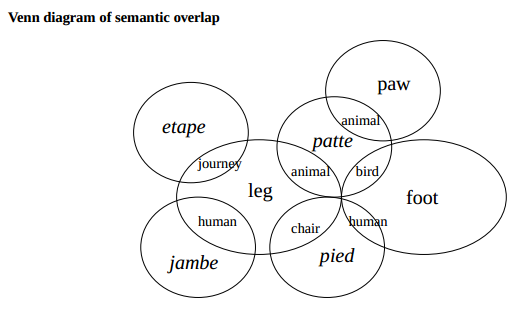
\includegraphics[width=12cm]{hutchins-leg-etc.png}
  \caption{Overlap of words related to ``leg"; relationships between English
  and French words. Translation is pretty complicated.}
  \label{fig:leg}
\end{figure}


%% XXX: this sentence needs some help
We will develop and extend at least two broad approaches for CL-WSD: the use
of multilingual evidence where available and sequence labeling.

Both of these techniques have been prototyped and presented at workshops, but
they will be refined significantly and integrated into a more general tool for
use in practice with MT systems.

\subsection{Using multilingual evidence}
For many languages, we have multiple bitext corpora, where each corpus covers a
different language pair. There are, for example, many bitext corpora available
for English and other languages, or for Spanish and other languages.
We would like to be able to make use of evidence from all of these corpora when
translating into any particular target language, if possible.
Each corpus may contain useful examples of a given source-language word,
and senses of that word may be lexicalized in varying, non-overlapping ways in
the different target languages.
We would want a CL-WSD system to be able to pick up on the relationships
between senses of a given word -- two target languages may happen to surface
the same sense distinctions, perhaps due to being related languages, or simply
by coincidence. Alternatively, a combination of translations into several
languages may provide evidence for a certain lexical choice in the target
language.

We could also imagine using a sense-annotated corpus to train a ``monolingual"
WSD system, and use this as a 
... basically ensemble methods for WSD.

This approach is informed by the work of Lefever and Hoste
\cite{lefever-hoste-decock:2011:ACL-HLT2011}, although their technique requires
an entire machine translation system to perform CL-WSD, which is somewhat
unwieldy when we want to use CL-WSD as a subcomponent of a machine translation
system.

Earlier this year, we developed a prototype CL-WSD system that makes use of
multilingual evidence \cite{rudnick-liu-gasser:2013:SemEval-2013} and produced
some of the best results in a SemEval shared task on CL-WSD \cite{task10}.
The task was to translate polysemous nouns from English into other European
languages. In our SemEval paper, we presented three variations on the approach:
a straightforward classification approach (without multilingual evidence), a
classifier stacking approach, and a graphical model system based on loopy
belief propagation over Markov networks.

The simplest system presented in that work, based on a maximum entropy
classifier, simply extracted features from a window around the English noun to
be translated and used these to make a prediction. The same system could also
return a probability distribution over target-language words or phrases. This
simple system was used as a subcomponent in the two more sophisticated systems.

The classifier stacking approach used 
for each available bitext corpus, for each source-language word that we want to
model, we train a classifier to predict translations from the source language
into the other language of the bitext.
Then we can include the output of that classifier as a feature when training
our classifier for the desired target language.


In the graphical model approach, we treat the problem of 
... this also has the property of explicitly handling the uncertainty of each
of the component classifiers.

\subsection{Lexical selection as a sequence labeling problem}
We will also investigate the use of sequence-labeling models for lexical
selection.  The intuition behind the sequence-labeling approach is that machine
translation implies an ``all-words" WSD task, in that we need to choose a
translation for every word or phrase in the source sentence, and that the
sequence of translations chosen should make sense when taken together.

One promising formalism for this line of work is the Maximum Entropy Markov
Model \cite{icml00/mccallum}, which can be combined in a straightforward way
with the simpler Hidden Markov Model (HMM).
This combination allows for efficient inference and the ability to trade more
computational resources for richer modeling. More sophisticated sequence
models, such as Conditional Random Fields, may be useful in this task as well.

We also developed a prototype CL-WSD system based on sequence labeling and
applied it to both English-Spanish and Spanish-Guarani translation tasks; this
work was presented at the HyTra workshop in August
\cite{rudnick-gasser:2013:HyTra-2013}.

For the sequence labeling approach in which only some words have their
translations modeled explicitly with a classifier, we have yet to explore what
the best approaches are for choosing \emph{which} words should get classifiers.

We will also look into the best ways to integrate the multilingual approach
with this one.

TODO look at the papers Nathan sent and be able to explain what other people
are doing for hard sequence labeling problems. That might go in the related
work section, or perhaps here.

\subsection{CL-WSD system combination}

Think about and expand the conversation I had with Markus.

You could imagine different CL-WSD systems rating each option separately and
then using MERT to get like an ensemble.
The question we were trying to address is like:
what if your n-gram model over labels for your source language has one idea
(this is the next likely label), and your emission probabilities say something
else (this is the label most likely to generate the observed input word)...
well, we could imagine just making several different decisions and letting the
decoder sort it out. We're doing that already actually, by including
phrase-table probabilities and a language model.
Are we just converging on the idea of a log-linear model again?
But the point here is that we don't have to have just one CL-WSD system. We can
have a bunch and let them fight it out. Hopefully this will help!

\subsection{Applying similar techniques for morphology prediction}

Sequence labeling has also been applied to the problem of generating
morphological features in target language text, so that target language output
words are appropriately inflected...
\cite{toutanova-suzuki-ruopp:2008:ACLMain}

This will be one of the approaches we investigate in the development of
Tereré...


\section{CL-WSD for Hybrid Machine Translation in Low-Resource Settings}
In recent years, we have seen renewed interest in machine translation systems
that take into account syntactic structure, linguistic knowledge, and semantic
representations.
Hopefully, these will provide better translation for language pairs with
significant reordering or syntactic divergences, and where one or both of the
languages has rich morphology.
The boundaries between rule-based and statistical MT systems are becoming
increasingly blurred, and hybrid systems are being developed in both
directions, with RBMT systems incorporating components based on machine
learning, as well as SMT systems making use of linguistic knowledge for
morphology and syntax.
Additionally, for most of the world's language pairs, there is simply no large
bitext corpus available, so training a purely statistical machine translation
system is infeasible.
Thus, while SMT approaches have had great success, and drastically changed the
machine translation landscape since the 1990s, RBMT approaches are still
relevant for many language pairs.

We would like for RBMT or hybrid systems, once developed, to be able to make
use of any bitext on hand.  Like SMT systems, they should be able to produce
better translations as larger corpora become available, without additional code
changes.

In this dissertation work, we will apply the CL-WSD techniques we develop to a
number of different MT systems with different designs, translating several
different language pairs.  These will include, at least: a hybrid SCFG-based
system that makes use of both bilingual transfer rules and a monolingual
language model, translating from Spanish to Guarani (Tereré) and a classic
transfer-based system translating Spanish to Quechua (Squoia).
We would also like to integrate into a more sophisticated RBMT system based on
constraint solving and synchronous dependency grammars (L3),
and a second system based on shallow transfer (Apertium), which has been
applied to a large number of language pairs.

\subsection{Tereré}
Since we hope that our ideas about lexical selection will make sense in several
different contexts, we will develop a new machine translation system out of
open-source SMT components, particularly relying on the cdec decoder and its
associated tools \cite{Dyer_etal_2010}.

This new system is called ``Tereré"
\footnote{\url{http://github.com/alexrudnick/terere}; 
Tereré is a cold variety of yerba mate brewed with ice water; it is a
specifically Paraguayan specialty.}.
Tereré will make use of modern hybrid MT techniques; our current design is
fairly similar to the Stat-XFER approach \cite{DBLP:conf/cicling/Lavie08}
developed by researchers at CMU.
Like Stat-XFER, Tereré will make use of bilingual transfer rules, a lexical
transfer stage, a target-language LM, and statistical decoding.

While the initial transfer rules will likely be written by hand, based the
respective grammars of Spanish and Guarani, we may also include
automatically-extracted rules, perhaps via Thrax \cite{weese-EtAl:2011:WMT} or
a forthcoming tool for extracting Inversion Transduction Grammars, from Dekai
Wu's team at HKUST \cite{saers-addanki-wu:2013:HyTra}.
The use of automatically-extracted transfer rules would make the system more
similar to the SAMT approaches of Zollmann and Venugopal
\shortcite{zollmann-venugopal:2006:WMT}.

In order to integrate our CL-WSD systems into Tereré, we will automatically
produce a SCFG rules just before decoding, in which features that encodes the
preferences of the WSD system are added to each lexical transfer rule. Then
the weights for all of the features provided to the system (translation
probabilities, LM scores, CL-WSD scores, and perhaps others) can be tuned with
MERT \cite{och:2003:ACL}, and the decoder will use these to search the space of
licensed translations.

We will approach the rich morphology of Guarani and the associated data
sparsity by having the system produce uninflected Guarani stems, which we will
then inflect in a second pass.
In the second pass, we will predict the appropriate morphological features will
with a discriminative sequence-labeling approach based on work at Microsoft
Research \cite{toutanova-suzuki-ruopp:2008:ACLMain}.
Thus both the transfer rules and the language model will be in terms of stemmed
Guarani.
As an alternative, we could adapt the techniques in
\cite{chahuneau:2013:emnlp} to generate translation rules that contain the
appropriately inflected target forms, just before running the decoder.
Rule-based approaches may also be sensible for generating Guarani morphology,
in some cases, and these will have to be investigated. In any case, once the
appropriate morphological features have been predicted, surface forms of
Guarani words will be generated with the FST-based morphological analyzer and
generator developed by Michael Gasser and described in
\cite{rudnick-gasser:2013:HyTra-2013}.

\subsection{SQUOIA}
SQUOIA\footnote{Described in detail at
\url{http://www.cl.uzh.ch/research/maschinelleuebersetzung/hybridmt_en.html}; 
Code available at \url{http://code.google.com/p/squoia/}}
is a project for MT from Spanish to Quechua, another relatively large
indigenous American language. SQUOIA is being developed by a team at the
University of Zurich. For the most part, it is a classical rule-based transfer
system, although the team has recently developed techniques for predicting verb
morphology with machine learning methods, in cases when rules cannot reliably
disambiguate \cite{riosgonzales-gohring:2013:HyTra}. It does not currently use
machine learning for lexical selection, although we have been in contact with
the team and are planning to collaborate to add CL-WSD features.

SQUOIA's architecture is based on the Matxin system \cite{matxin_2005}, which
was originally intended for translating from Spanish to Basque.
It consists of a pipeline of scripts, each of which passes along a tree
describing the current input sentence, in XML form. Adding CL-WSD to this
system will involve adding another script somewhere in the pipeline that
extracts features from the current annotated sentence, makes lexical choices,
and then passes these choices to subsequent scripts.

\subsection{L3}
L3 is an RBMT system based on synchronous dependency grammars and constraint
solving \cite{gasser:sxdg,gasser:aflat2012}.  It makes use of syntactic
knowledge about the source and target languages and can also include abstract
semantic representations as an intermediate stage in processing. Notably, L3
does not use a pipeline architecture: all of the constraints about the source
syntax, target syntax, semantic representation, and their relationships are
instantiated in one step, then solved jointly. L3 integrates morphological
analysis and generation for use in translating morphologically rich languages,
such as Guarani and Ethiopian semitic languages;
the morphological analyzers and generators to be used in Tereré were originally
developed for L3.

However, the constraints in L3 are currently unweighted, and it could use a way
to rank the licensed translations of an input sentence. It faces syntactic and
lexical ambiguity both in its analysis of the input sentence and in the
construction of output sentences. Ideally, a good lexical selection module
would constrain its other choices, yielding the higher-quality translations
first.

\subsection{Apertium}
Apertium\footnote{\url{http://www.apertium.org/}} \cite{Forcada_theapertium} is
another transfer-based RBMT system, originally designed for translating between
the languages of Spain but now handling over thirty language pairs. Some
language pairs are quite mature, while others are in prototype stages.

Apertium is a ``shallow transfer" system, meaning that it does not depend on
complete syntactic analysis of input sentences, but typically works by
chunking.
In his dissertation work (\cite{tyers-fst,tyers-thesis}), Francis Tyers has
been developing a new lexical selection system for Apertium, one that learns
lexical selection rules in the form of finite-state transducers from available
bitext. These rules are also human readable and editable, which seems like a
useful feature so that users can debug and tweak a translation system as
desired.
Tyers' lexical selection system is a strong baseline against which we should
compare our new CL-WSD approaches, and time and ingenuity permitting, we would
also like to integrate our system into Apertium.

\chapter{Data Sets, Tasks, Software and Evaluation}
\label{chap:evaluation}
In order to evaluate our CL-WSD approaches and their effects on translation
quality, we will need to have a basis for comparison between our proposed
techniques and sensible baselines, including results reported by other
researchers.

In this chapter, I describe the tasks and data sets that we will investigate
for the rest of the dissertation, as well as the basic version of the Chipa
software, which we extend in a variety of directions in the following chapters.

As discussed in Section \ref{sec:background-wsd}, for many years word sense
disambiguation systems have been evaluated \emph{in vitro} and in a monolingual
setting. The test sets for such WSD evaluations include sentences
hand-annotated with a word senses from a particular sense inventory, such as,
typically, the WordNet senses. These monolingual WSD evaluations often include
both coarse-grained and fine-grained distinctions and allow for several
possible correct answers; some word senses identified by lexicographers are
more closely related than others.  While the senses in a sense inventory will
contain many useful and interesting distinctions, they do not necessarily make
the distinctions most appropriate for a given task, wich will vary by
application. As such, accuracy improvements on these tasks do not necessarily
lead to performance gains for an NLP system making use of word-sense
disambiguations \cite{resnikwsdapplications}.

This style of evaluation relies on a fairly scarce resource: sentences
hand-annotated with a particular sense inventory.
In the CL-WSD setting, where we consider target-language lexical items to be
the salient senses of source-language words, we could also ask annotators to
hand-label each word of our test sentences with their translations.
For many language pairs, however, this annotation task has nearly been
performed by translators. We do not strictly have the labels for each token in
the source document, but with automatic word alignment techniques, we can infer
these labels with high confidence.

\section{Measuring MT Improvements}
We will additionally want to conduct \emph{in vivo} evaluations of our CL-WSD
techniques as applied to running MT systems. Here we can use standard
approaches for evaluating MT, such as BLEU and METEOR scores, or simply show
that where word choices differ with the application of CL-WSD, the changes are
for the most part improvements. For these experiments, we sample sentences
from the available bitext -- particularly sentences that contain polysemous
words for which we can train classifiers -- and run the MT systems both with
and without Chipa enabled.

We want to make the argument that improved classification accuracy on CL-WSD
tasks leads to improved translation results.
But in general, the addition of CL-WSD has not been an overwhelming success in
statistical machine translation, especially when we have large corpora
available for language modeling \cite{carpuatpsd}.
It seems intuitive that a
classifier producing correct word choices would lead an MT system to produce
better results. But we do not have a system that always indicates correct word
choices, nor are we likely to have one in the near future. And it is an
empirical question, whether the suggestions made by the CL-WSD system,
imperfect as they are sure to be, will improve translation results. We could
imagine gains failing to materialize, for example, if the CL-WSD system's
correct choices are mostly those that the MT system would have made on its own,
say with the guidance of a language model and phrase-table probabilities. 
We could even imagine its incorrect choices being misleading to the point of
doing harm to our translation quality.

These experiments are described in more detail in
Chapter~\ref{chap:integration}, where I also discuss how to integrate Chipa
into the different machine translation packages.

\section{Measuring CL-WSD Classification Accuracy}
One straightforward \emph{in vitro} approach for evaluating a CL-WSD system is
to measure classification accuracy over pre-labeled data. Here by
classification accuracy, we mean measuring how often the system is able to
correctly choose an appropriate translation for the focus word in a given
context.
Strictly speaking, we
do not have pre-labeled data: our bitext does not come with sub-sentential
alignments. But automatic word alignments provide a good approximation, as long
as our sentence alignments (or verse alignments, for Bible text) are accurate.
For the purposes of this work, we will assume that the automatic word-level
alignments are correct, putting in our best effort at preprocessing the
available text so that the aligner can produce useful output.

Using our automatically-aligned bitext as labeled data allows us to closely
mirror the lexical selection task faced by an MT system while translating
running text. We can train classifiers for many different word types, but we
will generally not have training examples available for all words in the input
at test time. This is a problem faced by data-driven NLP systems broadly.

For comparison with other work, in Section \ref{sec:baseline-semeval} we run
our systems on the SemEval CL-WSD shared task test sets, which are publicly
available.  Our larger task here is framed in the same way as the CL-WSD shared
tasks from 2010 and 2013, so measuring performance on these test sets allows a
straightforward comparison between the variations explored in this work and
several other CL-WSD systems from recent years. These test sets are limited in
scope, however, and will only demonstrate Chipa's performance for translating
individual English nouns. It is also worth noting that our more immediate
practical goal is to aid translation from Spanish into lower-resourced
languages. 

\section{Data Sets and Preprocessing}
The largest corpus that we have available for all of our source and target
languages is the Bible. There are translations available for many different
languages, and while these were not always produced by native speakers, the
translators are often driven by missionary zeal to produce high-quality
translations~\cite{DBLP:journals/lre/ResnikOD99}, so we can be reasonably
confident of the (linguistic) accuracy of our text.

In this work, we focus on one Bible translation per language. For Spanish, we
use the Reina-Valera translation (1995 edition), which I was able to scrape
from a Bible study website. Our Guarani translation, \emph{Ñandejara Ñe'e}
(1997 edition) was scraped from the same site. Our Quechua version (the 2004
translation published by the Peruvian Bible Society) was provided by Chris Loza
and Rada Mihalcea; the preparation of the Quechua corpus is described in Loza's
masters thesis \cite{chrisloza}. For English, we use the public domain World
English Bible translation.
While there are a large number of translations available online, different
``Bible societies" often own the associated copyrights and thus redistribution
of the complete texts is often restricted \cite{MAYER14.220.L14-1215}.

\subsection{Source-side annotations}
\label{sec:annotations}
In order to gracefully include a variety of features and build on
any available analysis tools for the source language, Chipa's input format and
feature functions allow for arbitrary annotations on source-language tokens.

Chipa's input file format describes one token per line, with fields split by
tabs.  The first field of a line is a token's lemma, and the second field is
its surface form. Following this are an arbitrary number of annotations for
that token, which may encode information such as part-of-speech, dependency
relations, or similar.  Sentence boundaries are indicated by blank lines. An
annotated sentence with one annotation per token might look like Figure
\ref{fig:quickbrownfox}, for example:

\begin{figure*}
\raggedright \texttt{\\
the	The	pos=DET \\
quick	quick	pos=ADJ \\
brown	brown	pos=ADJ \\
fox	fox	pos=NOUN \\
jump	jumped	pos=VERB \\
over	over	POS=ADP \\
the	the	POS=DET \\
lazy	lazy	POS=ADJ \\
sleep sleeping	POS=VERB \\
dog	dog	POS=NOUN \\
.	.	POS=. \\
  }
  \caption{Example annotated sentence.}
  \label{fig:quickbrownfox}
\end{figure*}

The Chipa software has been developed with a number of tools that consume and
produce this format, typically taking in sentences annotated in this way,
calling another NLP tool to generate more annotations, and then adding the new
annotations to those already present. The experiments in this chapter only use
one of these tools, \texttt{freeling\_to\_annotated.py}, which produces Chipa's
input format given output from Freeling.  In the following chapters, we will
make use of these tools and the extra information they make available to our
classifiers; in Chapter \ref{chap:monolingual} we add annotations learnable
with monolingual resources, and in Chapter \ref{chap:multilingual} we describe
tools and annotations that require parallel data.

\subsection{Preprocessing}
There is a nontrivial amount of preprocessing required in order to get our
Bible text into a format suitable for our tools.  This is largely due to the
varying markup formats used by different translation publishers.
For each of the available translations, we need to understand its formatting
enough to know which text comes from which book, chapter, and verse number.
This triple uniquely identifies a unit of text, and verse numbers are nearly
standardized across translations.  There are a few exceptions, however:
translations produced by different religious traditions may include different
books. Most notably, Catholic editions have a superset of the books found in
modern Protestant editions, and include slightly different chapters.
Additionally, in some translations, such as our Guarani edition, a few verses
have been combined into a single segment for a more natural translation.

In any case, if a particular book/chapter/verse is present in two Bibles, then
the two verses are very likely translations of one another. Once we find all of
the matching verses, we can build a bitext corpus suitable for use in our
pipeline.  In all four of our translations, we find all 66 books of the
Protestant Bible. Furthermore, we find matches for nearly all of the verses
across all of the language pairs considered. For English/Spanish and
Spanish/Quechua, the intersection of book/chapter/verse tuples across Bibles
contains over 99\% of the verses in any given Bible. For the Guarani
translation, however, we are only able to match 95.2\% of the verses. The
Guarani text contains fewer verses, $29,867$ versus the $31,104$ in Spanish,
showing that the translators were more willing here to combine verses and that
the translations may be more interpretive.

Our English translation is distributed in a format called USFM (Unified
Standard Format Markers), which is a markup language developed by a working
group of Bible translators and used widely by the Bible-related software
community; see Figure \ref{fig:usfmsample} for some sample input text in this
format.
\footnote{See \url{http://paratext.org/about/usfm} for more about USFM. USFM is
widely deployed; the website from which we scraped the Spanish and Guarani
corpora appears to render its HTML from a USFM source.  There is an entire
community of Bible software developers, and it has a wing that advocates Open
Source software and translations unencumbered by copyright.  One could delve
arbitrarily deeply into the history of religious-text translators and their
relationships with technology and copyright, but one has an NLP dissertation to
write.}
While there are a number of tools that consume USFM, I did not find one that
handles our particular use case of stripping metadata and simply mapping from
verses to flat text, so I wrote a short script, \texttt{parse\_usfm.py}, to
parse USFM and produce text in an easily-alignable format.

Our Spanish and Guarani corpora are extracted from HTML pages scraped from an
online Bible study website. In practice, the scraping was done by predicting
the URLs for each chapter of each book and requesting those URLs
programmatically. We then extract the text from the saved HTML pages with a
Python script and the BeautifulSoup library for HTML parsing.
\footnote{\url{http://www.crummy.com/software/BeautifulSoup/}}
As a side note, since websites change over time and we
downloaded the Guarani translation at an earlier date (from a mobile version of
the site that is no longer available), the HTML takes a significantly different
structure in the Spanish and Guarani editions, so they require different
versions of the script for preprocessing; see Figures \ref{fig:es-html-sample}
and \ref{fig:gn-html-sample} respectively for representative Spanish and
Guarani input.

Our Quechua translation came in an easily parseable format, with individual
verses already identified by Loza and Mihalcea; for this corpus, relatively
little preprocessing was necessary since lines begin with the book, chapter,
and verse already labeled. See Figure \ref{fig:loza} for a sample of the input
format.
It is conceivable that there are inconsistencies introduced by the
text-extraction processes for these different data sources, but for the most
part the scripts seem reliable, since they result in approximately the same
number of verses and tokens for our different languages, and the great majority
of the sentences are alignable (see subsequent discussion on bitext alignment).
Additionally, hand inspection of the text for the languages that I can
personally read (English and Spanish) show that the text contains fairly close
translations, and loan words and similar named entities appear in the Quechua
and Guarani texts.

\begin{figure*}
\raggedright \begin{verbatim}
\id LAM 25-LAM-web.sfm World English Bible (WEB) 
\ide UTF-8
\h Lamentations 
\toc1 The Lamentations of Jeremiah 
\toc2 Lamentations 
\toc3 Lam 
\mt2 The 
\mt Lamentations 
\mt2 of Jeremiah 
\c 1  
\p
\v 1 How the city sits solitary, 
\q2 that was full of people! 
\q She has become as a widow, 
\q2 who was great among the nations! 
\q She who was a princess among the provinces 
\q2 has become a slave! 
\b
\q
\v 2 She weeps bitterly in the night. 
\q2 Her tears are on her cheeks. 
\q Among all her lovers 
\q2 she has no one to comfort her. 
\q All her friends have dealt treacherously with her. 
\q2 They have become her enemies. 
\end{verbatim}
  \caption{The first two verses of the Book of Lamentations (World English
  Bible translation) in USFM format.}
  \label{fig:usfmsample}
\end{figure*}

\begin{figure*}
\raggedright \begin{verbatim}
[999,31,1,1] ¡Ay, imaraqmi Jerusalenqa sapan kapushan, haqay hina
  askha runakunayoq llaqta! ¡Ay, imaraqmi viuda warmi hina kapushan,
  lliw suyukunaq uman kashaqqa! Mit'anipina llank'apushan, lliw
  llaqtakunaq ñust'an kashaqqa.
[999,31,1,2] Tutan-tutanmi unuy-parata waqayku- shan, uyapas
  p'aspay-p'aspallaña. Llapan munaqninkunamanta manan hukllapas kanchu
  sonqochay- kuqnin. Llapan reqsinakuq-masinkunapas manan rikuqpas
  tukupunkuchu, llapallanmi awqanman tukupunku.
\end{verbatim}
  \caption{The first two verses of the Book of Lamentations in Quechua, from
  the 2004 Peruvian Bible Society translation. Whitespace changes added here
  for readability.}
  \label{fig:loza}
\end{figure*}

\begin{figure*}
\raggedright \begin{verbatim}
<div id="reader" class="content text_ltr">
  <a name="1"></a>
  <a href="/bible/more/Lam.1.1"
     style="color:black;text-decoration:none">
    <h2>El profeta </h2>
    <span class="verse" id="Lam_1_1">
    <strong class="verseno">1</strong>
    &nbsp;¡Pobrecita de ti, Jerusalén! <br />
    Antes eras la más famosa <br />
    de todas las ciudades. <br />
    ¡Antes estabas llena de gente, <br />
    pero te has quedado muy sola, <br />
    te has quedado viuda!  <br />
    ¡Fuiste la reina de las naciones, <br />
    pero hoy eres esclava de ellas! <br /> <p> </p></span>
  </a>
  <a name="2"></a>
  <a href="/bible/more/Lam.1.2"
     style="color:black;text-decoration:none">
    <span class="verse" id="Lam_1_2">
  <strong class="verseno">2</strong>
    &nbsp;Olvidada y bañada en lágrimas <br />
    pasas todas las noches. <br />
    Muchos decían que te amaban, <br />
    pero hoy nadie te consuela. <br />
    Los que se decían tus amigos <br />
    hoy son tus enemigos. <br />
    <p> </p></span>            </a>
\end{verbatim}
  \caption{The first two verses of the Book of Lamentations, \emph{Traducción en
  Lenguaje Actual} (TLA) version, in HTML as scraped from the web. Whitespace
  changes added here for readability.}
  \label{fig:es-html-sample}
\end{figure*}

\begin{figure*}
\raggedright \begin{verbatim}
<div class="ltr" data-abbreviation="gdc" data-reference="lam.1.gdc"
     data-usfm="LAM.1" id="version_primary">
    <div class="version vid66 iso6393nhd" data-vid="66"
         data-iso6393="nhd">
        <div class="book bkLAM">
            <div class="chapter ch1" data-usfm="LAM.1">
                <div class="label">1</div>
                <div class="s">
                    <span class="heading">Ñembyasy Jerusalén oñehundi
                    haguére</span>
                </div>
                <div class="q1">
                    <span class="content" />
                    <span class="verse v1" data-usfm="LAM.1.1">
                        <span class="label">1</span>
                        <span class="content">Ajépa ha'eño
                        ajejuhu</span>
                    </span>
                </div>
                <div class="q1">
                    <span class="verse v1" data-usfm="LAM.1.1">
                        <span class="content">upe táva
                        guasuete,</span>
                    </span>
                </div>
    ...
\end{verbatim}
  \caption{The beginning of the Book of Lamentations in Guarani,
  \emph{Ñandejara Ñe'e} version, in HTML as scraped from the web. Whitespace
  changes added here for readability. Note the metadata included here,
  suggesting that the HTML is generated programmatically from an underlying
  USFM document.}
  \label{fig:gn-html-sample}
\end{figure*}

Each of the different formatting schemes uses its own encoding to identify the
different books of the Bible, so when producing output for alignment, we must
map to a standard encoding. For example, our Quechua edition marks the book of
Lamentations with the numerical code $31$ (it is the thirty-first book in
modern Catholic editions), but in the USFM markup for the English translation,
we find a header with the string ``Lamentations". For our Spanish and Quechua
editions from the web, we find the code ``LAM" in the markup. In any case, we
map each of these identifiers to a single code ``Lam", so that we can match
books, chapters and verses across translations.

\subsection{Morphological Analysis}
\label{sec:guaranima}

For each of our languages, whether on the source or target side, in addition to
tokenizing, lowercasing and verse-alignment, we extract the lemmas (the
citation forms, normalized with respect to inflection) from each surface word.
Especially when working with smaller data sets and morphologically rich
languages, this is an important step; working primarily with lemmas rather than
surface-form words allows us to group, for example, the plural form of a word
with its singular.

For English and Spanish, we use the FreeLing suite of NLP tools
\cite{padro12} to extract lemmas. FreeLing provides a variety of analyses,
including tokenization, sentence splitting, multi-word expression and named
entity detection, part-of-speech tagging and parsing.  We start out using just
a few of these tools -- initially only tokenization and lemmatization. We
discuss making use of more of them in Chapter \ref{chap:monolingual},
leveraging the quality NLP tools that we have for our resource-rich source
languages.

The use of FreeLing for English is a noted improvement over initial
experiments, which used the WordNet lemmatizer and the default NLTK
part-of-speech tagger; these tools do not, as distributed, support Spanish.
The WordNet lemmatizer has a fairly small vocabulary, did not
provide a good strategy for dealing with unknown words, and could only address
nouns, verbs, and adjectives.
There are a very large number of named entities in the source text, most of
which are not present in WordNet. It cannot, by itself, help us know that
``Zebulonites" is the plural of "Zebulonite".  37\% of the tokens in our
English translation of the Bible are not present in WordNet, and many of these
tokens are function words. However, there are quite a few named entities in the
Bible: 33\% of the word types are not covered by WordNet either.

For Guarani and Quechua, we use Michael Gasser's ParaMorfo and AntiMorfo
analyzers.\footnote{Prof. Gasser's morphology software for Guarani, Quechua,
Spanish, and other languages is available at
\url{http://www.cs.indiana.edu/~gasser/Research/software.html}} Guarani text is
analyzed with ParaMorfo 1.1, and Quechua with AntiMorfo 1.2.  These packages
are based on software originally developed for Ethiopian Semitic languages
\cite{gasser:eacl09}, and use cascades of finite-state transducers (FSTs),
which is a common approach in morphological analysis \cite{beesley+karttunen}.
ParaMorfo and AntiMorfo use weighted FSTs to handle long-distance dependencies
between morphemes, but rather than having weights correspond to probabilities
to be combined with multiplication, the FSTs are weighted with feature
structures that are combined via unification. This approach was originally
introduced by Amtrup \cite{amtrup:03}. In an FST weighted with feature
structures, the result of a successful traversal is the unification of the
feature structure ``weights'' on the traversed arcs, as well as an output
string. All possible paths through the FST are searched, though many of these
paths will not lead to accepting states, or will fail due to unification
conflicts.  Because a feature structure is accumulated during the process of
transduction, each traversal through the transducer retains a memory of where
it has been, permitting the incorporation of long-distance constraints such as
those relating the negative prefix and suffix of Guarani verbs.

Here the result of morphological analysis of a word is a root and a feature
structure representing the grammatical features of the word.  For the basic
version of Chipa, we are only concerned with the lemmatized forms of the words
in our corpora, so we ignore the grammatical features for now.  In cases of
morphological ambiguity, which is to say cases where a surface form could be an
inflection of multiple distinct lemmas, we maintain this ambiguity rather than
trying to disambiguate from context.  The different possible lemmas are
separated by a slash; there are examples of this in
Figure ~\ref{fig:gn-qu-morpho-ambiguity}.

\begin{figure*}
\begin{itemize}
  \item Quechua: \emph{Llapan munaqninkunamanta manan hukllapas kanchu
  sonqochay- kuqnin.} is analyzed by AntiMorfo as \texttt{llapan
  munaqninkunamanta ma/mana huk/huklla ka/kanchu sonqochay - kuqnin}.
  \emph{manan} here could be an inflection of \emph{ma} 'certainly' or
  \emph{mana} 'no, none'. Similarly with \emph{huk} 'one, another one' /
  \emph{huklla} 'only, lonesome, single' and \emph{ka} 'yours' /
  \emph{kanchu} (a kind of bird).
  \item Guarani: \emph{Upe che ro'o ha upe che pire ombyaipa, umi che kãngue
  omopẽmba.} is analyzed by ParaMorfo as \texttt{upe
  che so'o ha upe che pire ombyaipa , umi che kã mopẽ/pẽ . }. Here
  \emph{omopẽmba} is ambiguous, and could be an inflection of \emph{mopẽ} 'to
  break (something)' or \emph{pẽ} 'to break (oneself)'.
\end{itemize}
\caption{Examples of morphological ambiguity in Quechua and Guarani,
having been run through AntiMorfo and ParaMorfo. The Quechua text is the first
sentence of Lamentations 1:2; the Guarani is Lamentations 3:4.}
\label{fig:gn-qu-morpho-ambiguity}
\end{figure*}

%% TODO "Did you run / are you planning to run another experiment where you
%force disambiguation? Either use the highest weights, or the first analysis
%..."
%% Force morphological disambiguation on the gn side, not a bad idea.

There are, of course, examples of morphological ambiguity in English and
Spanish. A familiar example from Spanish is that \emph{ir} 'to
go' and \emph{ser} 'to be' sharing their preterite-tense forms; this is a
fairly common phenomenon. However, the FreeLing analysis tools can typically
(heuristically) resolve these ambiguities for us, and in this work we assume
that the Freeling output is correct, or at least correct enough.

\subsection{Alignment}
As a precaution against verses that are not close translations, or perhaps have
combined several parts of the text together into one verse on only one side, we
run the cdec filtering tool (\texttt{filter-length.pl}) with its default
settings, which checks for unusual length disparities in the bitext. This ends
up removing roughly 7\% of the verses\footnote{Specifically, length filtering
removes $7.12\%$ of the verse pairs for Spanish-English and thus
English-Spanish, $6.69\%$ for Spanish-Guarani, and $6.72\%$ for
Spanish-Quechua.}, but manual inspection shows that those verses removed are in
general very loose translations, or that additional material is present on one
side.

Having tokenized, lowercased, verse-aligned and lemmatized, our corpora, we are
ready to extract word-level alignments.
For this we use the \texttt{fast\_align} tool from cdec
\cite{dyer-EtAl:2010:Demos}, with its default settings\footnote{With the
command given at \url{http://www.cdec-decoder.org/guide/fast_align.html}} and
the lemmatized text as input.
\texttt{fast\_align} runs several iterations of a variant of IBM Models 1 and
2, with a prior encouraging diagonal alignments
\cite{dyer-chahuneau-smith:2013:NAACL-HLT}.
While running, it tunes the parameters on the priors, and having learned a
translation model, outputs the single most likely one-to-many word alignments,
such that each source language token is linked with zero or more
target-language tokens in the corresponding verse.

%% XXX: should explain the difference between what fast_align is doing and the
%% basic Models 1 & 2.
%% TODO "explain? example?"
%% XXX: working here

\TODO{add a clear example alignment here, maybe a word aligned to a multi-word
expression}

\subsection{A deeper dive: producing Spanish-Guarani bitext}
To get a concrete idea about the process of producing our bitext and our
annotated source corpus, we will now step through the bitext production process
for our Spanish-Guarani language pair. For the precise process, please see the
source code
\footnote{\url{https://github.com/alexrudnick/terere/tree/master/bibletools}}.

We consider the ``raw materials" for this process to be the scraped Spanish and
Guarani bibles; see Figure \ref{fig:es-html-sample} for an example.  In order
to replicate this work, or to extend it to more languages, one will have to
acquire bitext covering one's preferred language. There are translations in
many different languages available on various Bible websites, however.

The result of the scraping process is a directory full of HTML files, the raw
HTML that was served by the Bible websites. For the sites that we scraped, each
chapter is served as an individual HTML file. From these HTML files, we must
extract the flat text of all of the available Bible verses.  We do this with
the \texttt{get\_verses.py}, a tool that uses BeautifulSoup to parse the input
HTML and navigate its structure, extracting the verse identifiers and verse
text as it goes. We call the output of \texttt{get\_verses.py} a ``Bible file";
it consists of tab-separated values, one per line, in which (book, chapter,
verse) tuples are paired with the text of those verses.

We then call the \texttt{print\_bitext.py} on pairs of Bible files. This script
finds matching verses (book, chapter, verse tuples) and produces bitext files
in the format expected by the cdec alignment tools, which is simply
source-language segments and target-language segments, separated by
\texttt{|||}. The output of \texttt{print\_bitext.py} is called
\texttt{bible.es-gn.unfiltered}, which contains some non-parallel "sentences"
and is untokenized. Individual sentences have not been preprocessed at all.

We then a filtering script from cdec, \texttt{filter-length.pl}, which filters
out segments where either side is too long, or where there is a large disparity
in length between source and target text, which indicates input segments that
are not close translations. After this filtering step, we have selected the
bitext from which we will train Chipa. See Sentences \ref{sent:wood-en} and
\ref{sent:wood-es} for an example of a pair of segments that is filtered by
this step. This is 1 Kings 18:33, and the beginnings of these segments clearly
have the same meaning; for the Spanish translation, though, the material in the
second sentence of the English text has simply been moved into the subsequent
verse (1 Kings 18:34) for whatever reason.

\begin{figure}
\enumsentence{
He put the wood in order, and cut the bull in pieces, and laid it on the wood.
He said, “Fill four jars with water, and pour it on the burnt offering, and on
the wood.”}
\label{sent:wood-en}
\enumsentence{
 Preparó la leña, cortó el buey en pedazos, lo puso sobre la leña,
}
\label{sent:wood-es}
  \caption{Segments filtered due to length disparity. Our English and Spanish
  versions of 1 Kings 18:33.}
  \label{fig:length-disparity}
\end{figure}

Given the sentence-aligned bitext corpus, which contains only the subset of the
source and target Bibles that we were able to verse-align (roughly, ``sentence
align", in more common MT terms, though a verse need not be a single sentence),
we now want to preprocess the source text to produce the annotated version used
for training. We call cdec's \texttt{cut-corpus.pl} to select just the source
side of the bitext, in this case the Spanish. Then we call Freeling to do basic
analysis on the input Spanish text: it provides tokenizing (for example,
splitting out punctuation adjacent to words), lemmatizing and tagging
\footnote{See the checked-in Freeling configuration file for the exact settings
used:
\url{https://github.com/alexrudnick/terere/blob/master/bibletools/freeling-config/es.cfg}}.
Then we run a Python script, \texttt{freeling\_to\_annotated.py}, to convert
the FreeLing output format into Chipa's source-language input format.

Now on the target language side, we do something analogous, although less
analysis of the target text is required, and Freeling does not support our
target languages. We again use \texttt{cut-corpus.pl} to select just the target
side, in this case the Guarani, and cdec's \texttt{tokenize-anything.sh} and
\texttt{lowercase.pl} to tokenize and lowercase the Guarani text. Then we run
Chipa's lemmatizer script over the Guarani text. It calls the Paramorfo
morphological analyzer on the Guarani tokens, producing Guarani lemmas. In
cases of morphological ambiguity, we produce tokens that maintain that
ambiguity, simply joining the possible lemmas with a slash.  Once lemmatization
is complete, we have produced the target-language lemmatized text.

Then we join together each line of the source-language lemmatized text with its
corresponding target-language lemmatized text, using cdec's
\texttt{paste-files.pl} script. The output of this is the sentence-aligned,
tokenized, lowercased, lemmatized bitext corpus, which is ready for word
alignment. To generate the word alignments, we call cdec's \texttt{fast\_align}
tool.

\begin{figure*}
\begin{tikzpicture}[scale=0.7]
  \tikzstyle{vertex}=[rectangle,rounded corners, fill=gray!80!white,draw=gray!70!black,
  minimum size=0.6cm,line width=1]
  \draw[step=1cm,draw=gray] (0,0) grid (10,13);

  \foreach \y/\f in {0/Amargamente, 1/llora, 2/en, 3/la, 4/noche, 5/y, 6/las,
  7/lagrimas, 8/corren, 9/por, 10/sus, 11/mejillas, 12/.} {
    \node[left] at (-.2,12.5-\y) {{\raggedleft \f }};
  }
  \foreach \x/\e in {
  0/Pyhare, 1/pukukue, 2/hasẽ, 3/{,}, 4/ha, 5/hesay, 6/mante, 7/hováre,
  8/osyry, 9/. } {
    \node[rotate=60,right] at (\x+.4,13.2) {{\raggedright \e}};
  }

  % draw word alignment
  \foreach \y/\x in {
  4/0, 4/1, 1/2, 3/3, 5/4, 7/5, 9/6, 11/7, 8/8, 12/9
  } {
    \node[vertex] at (\x+.5, 12.5-\y) {};
  }
\end{tikzpicture}
  \caption{A sample word alignment. The beginning of Lamentations 1:2, mapping
  from Spanish to Guarani. Alignment produced with \texttt{fast\_align}.}
  \label{fig:example-word-alignment}
\end{figure*}

After all of this preprocessing and alignment, we have produced three files of
interest to Chipa: first, we have the lemmatized bitext corpus. Second, we have
the one-to-many word alignments between the two sides of the bitext. These two
files taken together constitute the ground truth for the Chipa system -- the
source lemmas, and the subsequences of the target text that are considered to
be their translations. Note that these alignments could be NULL -- a source
word could correspond with an empty subsequence of target-language tokens. At
test time, we will want to predict those translations, whatever they happen to
be.

The third file contains the annotated version of the source text, which
includes all of the information of the source side of the preprocessed bitext,
in addition to the original surface forms and the annotations extracted from
FreeLing analysis. Further annotations can be added by other tools; in general,
annotated source-language corpora could contain whatever kinds of signals we
might like to add to aid classifiers in predicting translations. In Chapter
\ref{chap:monolingual}, for example, we discuss features learnable with
monolingual resources such as part of speech tags, Brown clusters, and
embeddings learned with neural networks. In Chapter \ref{chap:multilingual}, we
discuss features that require parallel corpora, such as CL-WSD predictions into
languages other than the current target language. But in all of these cases,
the additional features are passed to the classifiers via this
corpus-annotation approach.


\section{Exploring the Bitext}
\label{sec:exploring}
Even using only the Bible as bitext, we find a substantial number of
training examples for many of the most common word types, which, due to the
Zipfian distribution of word types in most texts, constitute a significant
fraction of the tokens exhibited. See Figures \ref{fig:mostcommon-lemmas} and
\ref{fig:mostcommon-surface} for more detail.
%% TODO: quantify this, per language!!
Some of these most common words
in the text are proper names or exhibit only one translation in the target
language, but for the most part we see, through the aligned bitext, that
the most common words are polysemous.
To take a few salient examples from the Spanish-English aligned text,
the verb \emph{hacer} can translate in a number of different ways: 'do',
'make', 'cause'; for \emph{decir}, we must choose between 'say', 'tell' or
'speak'; \emph{mujer} can mean either 'wife' or 'woman'; and \emph{reina} can
translate to 'reign' or 'queen'.  

\begin{figure*}
TODO: plot of rank of each word type versus the cumulative fraction of the text
covered by that word type. Do this for both surface forms and lemmas, for each
of en, es, qu, gn.
  \caption{Word ranks versus fraction of Bible tokens covered, for lemmas.}
  \label{fig:mostcommon-lemmas}
\end{figure*}

\begin{figure*}
TODO: plot of rank of each word type versus the cumulative fraction of the text
covered by that word type. Do this for both surface forms and lemmas, for each
of en, es, qu, gn.
  \caption{Word ranks versus fraction of Bible tokens covered, for
  (case-insensitive) surface forms.}
  \label{fig:mostcommon-lemmas}
\end{figure*}

There are analogous lexical ambiguities when translating from Spanish to
Guarani and Quechua.
For example, the Spanish \emph{pueblo} 'town' or 'people' can translate into
Quechua as \emph{llaqta} 'town/city', or \emph{runa} 'person'.
For translating from Spanish to Guarani, we see the verb \emph{volver}
'turn/return/repeat' translated as \emph{jey} 'again', but also as \emph{jere}
'turn'.

Figure~\ref{fig:mostcommon-en-es} gives the most common lemmas used in our
corpus for the four languages, along with their counts. In
Figure~\ref{fig:mostcommon-es-translations}, we see common lemmas from
Spanish along with their most likely translations into English, Guarani and
Quechua (as extracted from the bitext). For the purposes of this work, we will
consider words to be in-vocabulary if they appear at least fifty times in the
training corpus; we also do not include punctuation marks and stopwords (as
defined by the default NLTK stopword lists for English and Spanish) other than
common verbs.
%% XXX: magic number. Do we need to argue about fifty? What if we went down to
%% forty? Lower than that and this looks pretty ridiculous.

\TODO{update based on most recent preprocessing pipeline}

\begin{figure*}
  \begin{tiny}
  \begin{centering}
  \begin{tabular}{|r|c|c|}
    \hline
    rank & word type & count \\
    \hline
1 & be & 23542 \\
2 & have & 9389 \\
3 & say & 6664 \\
4 & yahweh & 6508 \\
5 & shall & 4413 \\
6 & god & 4112 \\
7 & come & 3603 \\
8 & son & 3303 \\
9 & go & 2985 \\
10 & do & 2799 \\
11 & king & 2744 \\
12 & one & 2547 \\
13 & israel & 2476 \\
14 & make & 2349 \\
15 & day & 2246 \\
16 & man & 2190 \\
17 & people & 2052 \\
18 & house & 2050 \\
19 & give & 1997 \\
20 & child & 1902 \\
21 & take & 1843 \\
22 & hand & 1793 \\
23 & father & 1782 \\
24 & land & 1758 \\
25 & men & 1518 \\
26 & also & 1456 \\
27 & let & 1386 \\
28 & bring & 1384 \\
29 & thing & 1375 \\
30 & lord & 1374 \\
31 & know & 1328 \\
32 & us & 1326 \\
33 & may & 1290 \\
34 & behold & 1289 \\
35 & city & 1233 \\
36 & therefore & 1220 \\
37 & word & 1195 \\
38 & speak & 1187 \\
39 & even & 1107 \\
40 & like & 1106 \\
41 & servant & 1073 \\
42 & name & 1060 \\
43 & see & 1037 \\
44 & offering & 1000 \\
45 & away & 1000 \\
46 & place & 993 \\
47 & david & 992 \\
48 & great & 936 \\
49 & among & 932 \\
50 & jesus & 930 \\
    \hline
  \end{tabular}
  \quad
  \begin{tabular}{|r|c|c|}
    \hline
    rank & word type & count \\
    \hline
1 & ser & 8436 \\
2 & haber & 8418 \\
3 & jehová & 6515 \\
4 & decir & 6006 \\
5 & hijo & 4955 \\
6 & dios & 4164 \\
7 & estar & 3925 \\
8 & hacer & 3872 \\
9 & tierra & 2832 \\
10 & rey & 2676 \\
11 & israel & 2445 \\
12 & hombre & 2418 \\
13 & tener & 2276 \\
14 & día & 2146 \\
15 & casa & 2056 \\
16 & dar & 2053 \\
17 & entonces & 2026 \\
18 & ir/ser & 1967 \\
19 & pueblo & 1918 \\
20 & pues & 1909 \\
21 & si & 1690 \\
22 & vosotros & 1623 \\
23 & así & 1597 \\
24 & mano & 1535 \\
25 & padre & 1521 \\
26 & señor & 1411 \\
27 & delante & 1292 \\
28 & ciudad & 1259 \\
29 & ver & 1241 \\
30 & poner & 1238 \\
31 & venir & 1182 \\
32 & palabra & 1178 \\
33 & tomar & 1105 \\
34 & cosa & 992 \\
35 & david & 976 \\
36 & responder & 957 \\
37 & mujer & 950 \\
38 & volver & 944 \\
39 & poder & 939 \\
40 & grande & 926 \\
41 & hermano & 912 \\
42 & ir & 904 \\
43 & corazón & 883 \\
44 & sacerdote & 873 \\
45 & lugar & 868 \\
46 & nombre & 867 \\
47 & salir & 833 \\
48 & sino & 831 \\
49 & hablar & 829 \\
50 & año & 823 \\
    \hline
  \end{tabular}
  \end{centering}
  \end{tiny}
  \caption{Some of the most common (lemmatized, non-stopword) word types in our
  English and Spanish Bibles}
  \label{fig:mostcommon-en-es}
\end{figure*}

\begin{figure*}
  \begin{tiny}
  \begin{centering}
  \begin{tabular}{|r|p{4.2cm}|p{4.2cm}|p{4.2cm}|}
    \hline
    es & translations (en)                    & translations (gn) & translations (qu) \\
    \hline
ser & be,  will be, it be, shall be              &   hína, niko, mba'e, ramo                                                              &  ka, kanqa, chayqa, kanki \\
haber & have,  there, i have, i                  &   vaekue, {\textlangle}hague, che, {\textlangle}ha'e                                   &  qan, chay, ma/mana, ni \\
%jehová & yahweh,  yahweh s, to, s                &  ñandejára,  jára, tupã, opa/pa                                                        & señor,  señor diosqa, señor diosmi, señor diospa \\
decir & say,  tell, speak, say to                &  'e,  'e ha'e, ha'e, 'e/ha'e                                                           &  ni, chaymi, hina/hinan, ni/nina/ninaku \\
dios & god,  lord, gods, yahweh                  &  tupã,  jára, momba'e, tupã jára                                                       &  diospa, diosqa, dios, diosmi \\
estar & be,  stand, now, behold                  &   \~{i}{i}, ime, hína, iko/ko                                                          &  ka/kasha, kasha, ka, kaq \\
hacer &  do, make, cause, he                     &   {\textlangle}japo, mba'e, haguã, japouka                                             &  ruwa, chay, ruwa/ruway, ruwa/ruwana \\
tierra & land, earth, ground,  country           &   yvy, {\textlangle}hetã, ko yvy, yvy ári                                              &  suyu, hallp'a, ka/kay pacha \\ %% , ka/kay \\
ir/ser & be,  go, come, depart                   &   ha, vaekue, upe, kuéra                                                               &  karqan, ri, ripu, hina/hinan \\
pueblo & people, among,  nation, multitude       &   {\textlangle}hetã, {\textlangle}hetã gua, opavave, israelgua                         & llaqta,  runa, llaq/llaqta, israel runa \\
pues &  for, therefore, so, then                 &   upe, niko, aipórõ, che                                                               &  chay, chaymi, chay hinaqa, chhaynaqa \\
si & if,  if you, but if, whether                &  ramo,  rire, ime, pende                                                               &  chayqa, ma/mana, chaypas, icha \\
así &  so, thus, this, therefore                 &   upe, péicha, kóicha, avei                                                            &  chay, ahi/ahina, chay hina, hina \\
%%padre & father,  parent, his father, father s    &  ru,  ru ypy, ypy, vaekue                                                              & tayta,  yaya, ñawpa tayta, tayta/taytay \\
padre & father,  parent, his father              &  ru,  ru ypy, ypy, vaekue                                                              & tayta,  yaya, ñawpa tayta, tayta/taytay \\
señor & lord, master,  sir, ruler                &  ñandejára,  jára, karai, che jára                                                     &  señor, apu, señorpa, señorníy \\
poner &  put, set, lay, make                     &   mo\~{i}{i}/\~{i}{i}, mo\~{i}{i}, mo\~{i}{i}/ñemo\~{i}{i}/\~{i}{i}, upéi              &  chura, hina, hinaspa, chay \\
%venir & come,  will come, behold, will           &   ju, guah\~{i}{i}{e}, aju/ju, rendápe                                                 &  hamu, chaya/chayamu, hamu/hamuq, chaya \\
%tomar & take,  shall take, took, he take         &   raha, momba'e, {\textlangle}hupi, japyhy                                             &  hap'i, hina, hina/hinan, apa \\
%responder & answer,  say, then, but              &  'e,  'e ha'e, katu, katu 'e                                                           &  kuti/kutichi, ni, chaymi, hina/hinan \\
mujer & woman, wife,  a wife, a woman            &  kuña, {\textlangle}hembireko,  menda, kuñakarai                                       & warmi,  war, warmi/warmiy, qhari \\
volver & return,  turn, again, back              &   jey, jeýta, ju jey, jere                                                             &  kutipu, wakmanta, kuti, kuti/kutimu \\
poder & can,  power, able, could                 &  katu,  pu'aka, ndaikatu, mbarete                                                      &  ati, ati/atiy, ma/mana, atiyniyoq \\
ir & go,  come, will, let                        &   ha, s\~{i}{i}{e}, ha ha, {\textlangle}hasa                                           &  ri, ripu, ri/rina, ri/risa \\
%% lugar & place,  instead, in, place where         &   {\textlangle}henda, {\textlangle}hendague/{\textlangle}hendaguépe/hendague, {\textlangle}henda/ha'e, {\textlangle}hendague/{\textlangle}hendaguépe/rendague  &  ranti, cheqasta, ma, cheqasman \\
salir & go out, come out,  out, go               &  s\~{i}{i}{e},  upe, ha, s\~{i}{i}{e} okápe                                            &  ri, lloqsispa, puriri, hina/hinan \\
%siervo & servant,  slave, male servant, young    &  {\textlangle}hembiguái,  mburuvicha, che, {\textlangle}huvicha                        &  kamachi, kama/kamachi, kama/kamachi/kamachiy, kama \\
judá & judah, jew,  belongs, of judah            &  judá, judagua,  judápe, judágui                                                       & judá, judá suyu,  judapi, judá ayllu \\
mismo &  same, himself, own, myself              &   voi, avei, upe, pete\~{i}{i}                                                         &  kikin, kaq, chay, hina/hinalla \\
% oír & hear, heard, listen,  when                 &  {\textlangle}hendu,  kuaa, {\textlangle}hendu/ndu, japysaka                           & uyari,  uya, uyari/uyarina, uyari/uyariqkuna \\
llevar & bring,  carry, take, bear               &  raha,  {\textlangle}hupi, raha hikuái, hikuái                                         &  apa, pusa, apa/apamu, apari/apariku \\
% hecho & do,  make, done, work                    &   {\textlangle}japo, {\textlangle}japo vaekue, {\textlangle}hembiapo, mba'e            &  ruwa, ru, kama, allinta \\
dicho & say, speak,  tell, word                  &  'e,  'e/ha'e, kóicha 'e, {\textlangle}he'ika                                          & ni,  diosmi ni, apu, diosmi \\
cielo & heaven, sky,  heavens, cloud             &  yvága,  ára, yvate, yvága pe/pegua                                                    & hana/hanaq pacha,  pacha, hana/hanaq, hana/hanaq pa \\
ojo & eye, sight,  in, his eye                   &   {\textlangle}hesa, {\textlangle}hecha, ma'\~{i}{i}{e}, che                           &  ñawi, qhawari, ri/riku, ruwa \\
llegar & come,  have come, reach, when           &  guah\~{i}{i}{e},  guah\~{i}{i}{e} hikuái, ke, ja/mboja/ñemboja                        &  chaya, chaya/chayamu, hamu, cha \\
%quedar & be,  stay, remain, be leave             &   pyta, {\textlangle}hemby, {\textlangle}heja, ndopyta                                 &  kapu/kapun, kanqa, qhepaq, qhepakurqan \\
%aquel & that,  him, will, everyone               &  upe,  pe, upe upe, umiha                                                              & chay,  pipas, haqay, chaypachan \\
%% cada & each, every,  everyone, every man         &   te\~{i}{i}, opa/pa, {\textlangle}he\~{i}{i}/{\textlangle}he\~{i}{i}me/te\~{i}{i}, pete\~{i}{i} te\~{i}{i}    &  sapanka, sapa, sapa/sapan, sapankanku \\
% medio &  middle, among, through, within          &   rupi, mbytépe, apytépe, pende                                                        &  ukhu, ukhupi, chawpi, qankuna \\
entrar & enter into, come, come into, go into, go&  ke,  guah\~{i}{i}{e}, ndoike, hikuái                                                  & hayku,  hayku/haykuna, ri, hay \\
%% llamar & call, name,  whose name, summon         &  {\textlangle}héra, {\textlangle}henói,  {\textlangle}henoika/henoika, {\textlangle}henói/nói                                          &  waq/waqya, sutiyoq, waqya, suti/suticha \\
llamar & call, name, summon                      &  {\textlangle}héra, {\textlangle}henói,  {\textlangle}henoika/henoika, {\textlangle}henói/nói                                          &  waq/waqya, sutiyoq, waqya, suti/suticha \\
%espíritu & spirit,  breath, by, trouble          &  espíritu,  espíritu santo, py'a, pu'aka                                               &  santo espirituq, santo, espiritun, santo espirituqa \\
%monte & mountain, on,  mount, hill country       &  yvyty,  yvyty {\textlangle}hu'ã, ka'aguy, yvyty rupi                                  & orqo,  orqopi, orqoman, orqokuna \\
subir & go up, come up, up,  ascend              &   jupi, ha, s\~{i}{i}{e}, ju                                                           &  wicha, ri, wichari, chay/chayman \\
obra & work, do,  deed, doings                   &   {\textlangle}hembiapo, {\textlangle}japo, mba'e, mba'e {\textlangle}japo             & ruwa,  llank'a, ruwa/ruwana, ruwa/ruway \\
%% puerta & gate, door, at,  threshold              &  {\textlangle}hok\~{i}{i}{e},  k\~{i}{i}{e}, táva {\textlangle}hok\~{i}{i}{e}, {\textlangle}hok\~{i}{i}{e} nguéra          & punku,  hayku/haykuna, punku/punkuta, pun \\
% pecado & sin, iniquity, trespass,  transgression &  angaipa,  {\textlangle}hembiapo vai, vai, {\textlangle}heja rei                       & hucha, huchalli/huchalliku,  hucha/huchaku, hu \\
hija & daughter,  her, her daughter, woman       &  rajy,  kuña, memby, táva                                                              & ususi,  warmi, warmi wawa, llaq/llaqta \\
% junto & by,  together, beside, at                &   {\textlangle}hembe'y, ypýpe, ykére, \~{i}{i}                                         &  qaylla, patapi, kuska, qayllapi \\
dejar & leave,  let, allow, they                 &   {\textlangle}heja, poi, ja, jei                                                      &  kachari, ama, ma/mana, maña/mañana \\
    \hline
  \end{tabular}
  \end{centering}
  \end{tiny}
  \caption{Selected common Spanish word types with their most likely
translations. These were picked for interesting polysemy from the 100 most
common word types.}
  \label{fig:mostcommon-es-translations}
\end{figure*}

\begin{figure*}
  \begin{tiny}
  \begin{centering}
  \begin{tabular}{|r|c|c|c|c|}
    \hline
    es & entropy (en) & entropy (gn) & entropy (qu) \\
    \hline
ser    &     2.49         &      3.90        &       3.25       \\  
haber  &     2.88         &      3.57        &       2.70       \\
decir  &     1.57         &      2.05        &       1.82       \\
dios   &     0.33         &      1.56        &       3.99       \\
estar  &     2.07         &      3.01        &       2.61       \\
hacer  &     4.07         &      2.68        &       2.67       \\
tierra &     2.00         &      2.96        &       3.58       \\
ir/ser &     2.65         &      3.19        &       2.92       \\
pueblo &     0.56         &      3.36        &       3.21       \\
pues   &     3.18         &      3.73        &       2.90       \\
si     &     2.68         &      3.06        &       2.91       \\
así    &     2.95         &      2.73        &       3.27       \\
padre  &     0.53         &      1.48        &       2.60       \\
señor  &     0.78         &      3.15        &       3.38       \\
poner  &     4.32         &      3.05        &       2.93       \\
mujer  &     2.11         &      2.28        &       1.88       \\
volver &     3.89         &      3.59        &       3.65       \\
poder  &     3.51         &      3.12        &       3.36       \\
ir     &     3.49         &      2.96        &       2.77       \\
salir  &     3.43         &      2.40        &       3.91       \\
judá   &     0.23         &      2.07        &       2.81       \\
mismo  &     3.27         &      2.94        &       2.87       \\
llevar &     3.70         &      1.81        &       2.79       \\
dicho  &     1.91         &      2.60        &       2.99       \\
cielo  &     1.32         &      2.21        &       2.13       \\
ojo    &     2.03         &      2.52        &       2.57       \\
llegar &     3.23         &      2.76        &       3.27       \\
entrar &     3.77         &      1.88        &       2.71       \\
llamar &     1.64         &      2.69        &       3.49       \\
subir  &     2.85         &      3.39        &       3.19       \\
obra   &     1.99         &      3.27        &       3.42       \\
hija   &     0.35         &      2.33        &       2.29       \\
dejar  &     4.03         &      2.67        &       2.80       \\
    \hline
  \end{tabular}
  \end{centering}
  \end{tiny}
  \caption{Common Spanish word types and the entropy, in bits, faced by a
  system that must choose among the possible alternatives} 
  \label{fig:mostcommon-es-entropy}
\end{figure*}
%% TODO "I did not find a mention / explanation of this figure in the text."


Using larger bitexts of course will allow us to construct training and test
sets for a broader vocabulary, and with better statistical support for the
words already present. However even when working with the Bible, we
have at least fifty uses of over a thousand different lemmas, for English and
Spanish, as shown in Figure \ref{fig:mostcommon-en-es}.

\TODO{For comparison, do we want to include the stats for Europarl here too? Or
maybe we could put that in the ``multilingual" chapter?}

\section{Baseline Chipa System}
At its core, the Chipa software takes in a word-aligned bitext corpus, with
annotations for the source tokens. It then trains CL-WSD classifiers for
source-language word types on demand. 

The software holds all of the available bitext in memory. On request, it
constructs a training set for learning to disambiguate a given word
by retrieving all sentences that contain that word,
finding the instances of that word and its aligned translations, and extracting
features (see Figure~\ref{fig:baselinefeatures}) from the source side and its
annotations.
If a source-language word has been seen aligned to only one target-language
type, then this is simply noted, and if the source word is not present in the
training data, then that word is marked as out-of-vocabulary. In these two
cases, we do not train a classifier for that word, since there is no
ambiguity present in our examples and the Chipa software cannot provide any
useful guidance to its caller. A machine translation system may, for example,
refuse to translate sentences with OOV words, or more likely, will simply
assume the identity translation, effectively passing them through untranslted.

Since source-language tokens may be NULL-aligned (i.e., not all words in the
source text will have corresponding words in the target text), both in the
training data and in translations, Chipa provides the option to request
classifiers that consider NULL as a valid label for classification, or not, as
appropriate for the translation application. We here report classification
accuracies for both settings.

Memory permitting, Chipa classifiers are kept cached for later usage. Chipa can
also be run as a server, providing an interface whereby client programs can
request CL-WSD decisions over remote procedure calls (RPC).

Chipa's classifiers are trained with the scikit-learn machine learning toolkit
\cite{scikit-learn} for Python and its associated NLTK interface, though in
earlier versions, we used the megam package \cite{daume04cg-bfgs}, also through
NLTK. By default, we use Logistic Regression classifiers (also known as
Maximum Entropy), with the default scikit-learn settings.
Maximum entropy classifiers are well-suited to this sort of classification
task, as they are robust to adding large numbers of features, even
highly-correlated ones \cite{nigam1999using}. Here we have exactly this
situation, large numbers of sparse features, where some of them are likely to
be highly correlated, since our features contain several representations of the
tokens from the input sentence -- their surface forms and their lemmatized
forms, and the presence of a word in the window surrounding the focus word
guarantees its presence in the bag of words representing the entire sentence.
This is fairly typical of text classification problems.

Furthermore, because we have a large number of features but a relatively small
number of samples per classifier, we train with L1 regularization rather than
L2~\cite{ng2004feature}.
We can also set a regularization parameter during training, to encourage
more parsimonious solutions and thus avoid overfitting.
Here by default we set the regularization parameter to $C=1.0$.
%% TODO "If the results were worse, you can just report this in one sentence."

We have also tried a variety of classification algorithms; scikit-learn makes
experimentation with different classifiers and parameter settings
straightforward. We have tried random forests and linear support vector
machines, and of course compare these to the most-frequent-sense baseline.

\TODO{Report results with a few different regularization settings}
\TODO{Report results with SVMs and random forests too.}

\begin{figure*}
  \begin{centering}
  \begin{tabular}{|r|p{11cm}|}
    \hline
    name          & description  \\
    \hline
    \texttt{bagofwords}    & a feature counting each lemma in the source sentence \\
    \hline
    \texttt{bagofsurface}  & like \texttt{bagofwords}, but with surface forms \\
    \hline
    \texttt{window}       & a binary feature for each of the lemmas in the immediately surrounding three-word context window \\
    \hline
    \texttt{surfacewindow} & like \texttt{window}, but with surface forms \\
    \hline
  \end{tabular}
  \end{centering}
  \caption{Features for the baseline Chipa system}
  \label{fig:baselinefeatures}
\end{figure*}

\section{Classification Results for the Baseline System}

\TODO{insert a bunch of numbers here}

\begin{itemize}
\item en-es
\item es-en
\item es-gn
\item es-qu
\end{itemize}

\TODO{Words in Spanish for which we gain the most by training a classifier --
measured as the difference in accuracy between MFS}

\section{For Comparison: the Baseline Chipa System On the SemEval 2010 and 2013
Shared Tasks}
\label{sec:baseline-semeval}
\TODO{this means we have to actually run the latest Chipa on the SemEval test sets too}
%% """if you end up using these data set for evaluation, I'd like to see
%information here about how the data were annotated, where the translation
%candidates came form, how big the data sets were ""


\urldef{\leydelenguas}\url{http://www.cultura.gov.py/lang/es-es/2011/05/ley-de-lenguas-n%C2%BA-4251/}

\chapter{Paraguay and the Guarani Language}
Guarani is an indigenous language spoken in Paraguay and the surrounding
region.
Historically, it was the native language of the indigenous Guarani people. The
word for the Guarani language in Guarani is \emph{avañe'e} (``people's
language", where \emph{ñe'e} means ``language").

Guarani is unique among indigenous American languages in that a substantial
number of non-indigenous people speak it.  The majority of Paraguayans are
conversant in Guarani, although they are likely to be bilingual with Spanish.
In practice, many Paraguayans use a combination of Guarani and Spanish called
\emph{Jopar{\'a}}, which is the Guarani word for ``mixture".

Paraguay is officially a bilingual, pluricultural country, as described by its
famous \emph{Ley de Lenguas} \footnote{\leydelenguas} (``Law of Languages").
However, the Guarani language is at a significant social and economic
disadvantage and is typically not used in formal situations, as Spanish is
often considered more prestigious. There are, however, an engaged activist
community, many Guarani-language educators, and a government agency devoted
specifically to policy regarding language.
The Guarani language figures significantly into a sense of Paraguayan national
identity and history.

Guarani has a rich, polysynthetic, agglutinative morphology, in which roots can
derive into different parts of speech, and often several roots can combine into
a single word. Guarani morphology can mark tense, aspect (even on nouns),
number, negation, and other features. However, unlike Spanish, it has no
grammatical gender.  Guarani's rich morphology can make many NLP tasks,
including ones seemingly as simple as spell-checking, rather challenging.

We are in contact with a number of collaborators in Paraguay, including
language activists and educators from the \emph{Ateneo de la Lengua y Cultura
Guaraní} \footnote{\url{http://www.ateneoguarani.edu.py/}} and the
\emph{Fundación Yvy Marãe'{\~y}} \footnote{\url{http://yvymaraey.org/}},
both of which are schools that offer training for Guarani-language translators.

We have also started discussing development plans with several local software
developers -- including some from the local One Laptop Per Child organization
-- interested in building open source software, such as the corpus-building
websites described in the next section.

\section{Acquiring larger bitext corpora}
As part of the ongoing work for the practical goal of building a useful
Spanish-Guarani MT system, we would like to build larger training corpora,
containing both bitext and monolingual Guarani text.
To help in the collection, we plan to build two websites:
a collaborative online space for building translations of documents, 
and a searchable repository of Guarani and bilingual documents.
Initial designs for both of these sites were done as a master's project in HCI
by Alberto Samaniego\footnote{\url{http://albsama.com}}, who will hopefully
continue collaborating on this project from his native Paraguay.
We have also had helpful software contributions from
Rodrigo Villalba Zayas\footnote{\url{https://github.com/rodrigovz}} --
also from Paraguay -- and more potential collaborators have expressed
interest in helping, from Paraguay, Indiana, and the broader open-source world.

\subsection{Collecting Guarani Documents}
The first website we will develop is called ``Tahekami", which means
\emph{let's search together} in Guarani.
Tahekami is a repository of Guarani and bilingual documents that will allow
searching, browsing documents by tag, and uploading new documents.

An initial version of this site is already well underway
\footnote{\url{http://github.com/hltdi/gn-documents}}.  We have a working
search engine based on the Whoosh library
\footnote{\url{https://bitbucket.org/mchaput/whoosh/wiki/Home}} and some sample
documents -- twelve masters theses from the \emph{Ateneo}. We will need to
develop policies for which documents are permissible for distribution through
this site and work on integrating morphological analysis into the search
engine. Currently, new documents must be approved by an administrator before
being added to the index.

\subsection{Collecting Translations}
The second website, tentatively called ``Guampa"
\footnote{A ``guampa", in Paraguay, is the cup from which one drinks yerba mate
or tereré. The term ``guampa" is also local to Paraguay; in other parts of
South America, the container itself is called a ``mate".},
will be used by Guarani speakers and learners to produce translations of
relevant documents from Spanish to Guarani or vice-versa.
It will be something like a bilingual wiki, although the interface will
encourage users to edit sentences individually.
The software will segment the sentences in the initial
source-language documents and allow users to contribute translations for each
source sentence in turn, while showing the complete document context.
As a result of this, not only will will we be able to collect bitext training
data, but we will also produce useful translations.

Initially, this site will be seeded with documents from the Spanish and Guarani
Wikipedias. Successful translations of the Spanish-language articles could be
fed back into the Guarani Wikipedia. Other documents will be added by
Guarani-language educators and perhaps also pulled from Tahekami. Translations
may be assigned as homework by Guarani-language teachers.

The website will keep track of translations contributed by individual users;
there may be game-like features and community voting, where large number of
translations, or particularly good ones, are recognized, perhaps with virtual
prizes and badges.
Ideally, community management will be addressed by Paraguayan volunteers and
the gamification features can be built by contributors from the open source
world; this website and its richer features are not the primary focus of this
dissertation.

We may eventually collect enough bitext with this website such that it makes
sense to develop approaches for determining which sentences are the most
reliable and the most useful for training; this may correlate with quality
judgements from the human volunteers.
Investigating this relationship would make a good research question.

In the medium-term, this website will get an integrated ability to search
a translation memory and automatic suggestions from a machine translation
system\footnote{Features described in a presentation in Spanish here:
\url{http://www.cs.indiana.edu/~gasser/Taller2013/} ; English-language similar
presentation: \url{http://tinyurl.com/alexr-clingding-guarani} }
. While these features will be both useful and present a number of
interesting research questions, they are outside the scope of this
dissertation.

\section{Related Work}
\label{sec:relatedwork}

\subsection{Cross-lingual Word Sense Disambiguation}

While most SMT systems do not make use of an explicit WSD module, recently
Carpuat and Wu have shown how to use word-sense disambiguation techniques to
improve modern phrase-based SMT systems, in a normally 

\cite{carpuatpsd,carpuat-wu:2007:EMNLP-CoNLL2007,carpuat2008evaluation}


ParaSense, the system of Lefever
and Hoste, takes into account evidence from all of the available parallel
corpora. Let $S$ be the set of five target languages and $t$ be the particular
target language of interest at the moment; ParaSense creates bag-of-words
features from the translations of the target sentence into the languages $S -
\lbrace{t \rbrace}$.
Given corpora that are parallel over many languages, this is straightforward at
training time. However, at testing time it requires a complete MT system for
each of the four other languages, which is computationally prohibitive. Thus in
our work, we learn from several parallel corpora but require neither a locally
running MT system nor access to an online translation API.

Following the work of Lefever and Hoste
\shortcite{lefever-hoste-decock:2011:ACL-HLT2011}, we wanted to make use of
multiple bitext corpora for the CL-WSD task.

To our knowledge, there has not been other work on framing all-words WSD as a
sequence labeling problem. However, in monolingual WSD, Molina \textit{et al.}
\shortcite{DBLP:conf/iberamia/MolinaPS02}
have made use of HMMs for WSD. 


\subsection{Translation into Morphologically Rich Languages}



Chris Dyer's recent paper at EMNLP
\cite{chahuneau:2013:emnlp}

Talk about prediction for morphology.
\cite{toutanova-suzuki-ruopp:2008:ACLMain}

Also factored models...
\cite{yeniterzi-oflazer:2010:ACL}

\subsection{Hybrid Machine Translation for Under-Resourced Languages}
HMT for low-resource languages...

%% text from the HyTra paper
However, there has been work recently on using WSD techniques for translation
into lower-resourced languages, such as the English-Slovene language pair, as
in \cite{vintar-fivser-vrvsvcaj:2012:ESIRMT-HyTra2012}. 

The Apertium team has a particular practical interest in improving lexical
selection in RBMT; they recently have been developing
a new system, described in \cite{tyers-fst}, that learns finite-state
transducers for lexical selection from the available parallel corpora. It is
intended to be both very fast, for use in practical translation systems, and
to produce lexical selection rules that are understandable and modifiable by
humans.

Put in some stuff about SAMT and Stat-XFER.

Who's doing transfer rules that are hand-written?


\subsection{Creating Corpora Through Crowdsourcing}
There has been some work on creating multilingual corpora through
crowdsourcing, in several variations. Some projects have explicitly had the
goal of creating sentence-aligned bitexts useful for training MT systems, while
others have aimed to create useful resources for humans. Also the means of
crowdsourcing has varied; some contributors have been paid, and others are
volunteers.

Vamshi Ambati's recent work \cite{ambati_naacl,ambati_act} focuses on using
crowdsourcing and active learning to produce a corpus for English-Spanish SMT.
His system has a representation of which words and phrases it should learn
about, finding n-grams that are common in a development set but have little
support in the training set, and then automatically creates Mechanical Turk
tasks to elicit translations containing translations of these n-grams. This
work makes use of the relatively large population of Internet users (and thus
MTurk users) familiar with both English and Spanish, and succeeded in building
a large bitext corpus quickly and cheaply.

The Joshua team at Johns Hopkins has also successfully used Mechanical Turk to
crowdsource the creation of corpora for SMT
\cite{post-callisonburch-osborne:2012:WMT}. In this work, the team built
large parallel corpora for many languages of the Indian
subcontinent\footnote{\url{http://joshua-decoder.org/indian-parallel-corpora/}}
and developed a simple approach for discovering the high-quality contributions,
in which MTurk users vote on which translations they consider the best.

There's also MonoTrans
\url{http://www.cs.umd.edu/hcil/monotrans/}
"... an iterative protocol in which monolingual human participants work
together to improve imperfect machine translations." 

Contrastingly, the Tatoeba project is a repository of 
%% Tatoeba
Tatoeba -- repository of a bunch of example sentences translated into a variety
of languages.
\url{http://tatoeba.org/}

%% Tradubi
Tradubi project
\url{http://wiki.apertium.org/wiki/Tradubi}

(project seems to have died, though)

%% Traduwiki
Traduwiki
\url{http://traduwiki.org}

This looks awesome. If we could just bring up an instance of this, that would
be close to the right thing.

%% OPUS
OPUS, "the open parallel corpus".
\url{http://opus.lingfil.uu.se/}

\subsection{Online Language Tools for Guarani}

While there are not currently many online language tools for the Guarani, there
are a few ...

Notably, there is 
iGuarani
\url{http://iguarani.com/}

Wolf Lustig's dictionary
\footnote{\url{http://www.uni-mainz.de/cgi-bin/guarani2/dictionary.pl}}, which
has versions in Spanish, German, and English.


\footnote{\url{http://cafehistoria.ning.com/profiles/blogs/la-lengua-guarani-o-avanee-en}}

\section{Research Plan}

In the coming year, we have a large -- but finite -- number of tasks that we
would like to perform to carry out this dissertation work. What follows is a
rough, tentative list of the tasks, with their timeline.

\begin{itemize}
  \item Bring up initial versions of the Tahekami and Guampa websites in
  October 2013, in time for the LREC deadline. We will write an LREC paper
  about Guampa at least.
  \item Ongoing development of the data-collection websites should (ideally)
  largely be handled by open-source volunteers, from Indiana and Paraguay.
  \item Development of the various CL-WSD approaches will be ongoing and
  modular.
  \item Before the EACL short-paper deadline (January 2014), we should have
  packaged up a more modular CL-WSD system and integrated it into the SQUOIA
  system (Spanish-Quechua RBMT from Zurich) at least.
  \item Development of Tereré, the SCFG-based hybrid system, will be ongoing,
  but hopefully it will be prototyped by the end of 2013 and useful by Spring
  semester 2014.
  \item Experiments and evaluation will be underway by Spring semester 2014.
  \item Dissertation writing will be ongoing, but hopefully finishing up by
  Summer 2014.
  \item Thesis Defense by September 2014.
\end{itemize}

\section{Status and Expected Contributions}

Thus far, we have prototyped our CL-WSD systems that make use of multilingual
evidence and sequence labeling techniques and seen promising initial results
with these approaches, as described in \S\ref{sec:clwsd} and our papers
mentioned in that section.

Initial experiments are underway with building Tereré on top of the cdec
toolkit; we can already train Guarani-language LMs with KenLM
\cite{Heafield-estimate}, trained on the Guarani-language Wikipedia.
Additionally, we have mocked up the inclusion of CL-WSD features into the
decoder and started experimenting with writing SCFG transfer rules.

The Tahekami website is already well underway, and we have a web server on
which we can run Tahekami and Guampa. Fairly enthusiastic volunteers, including
developers from Paraguay, will likely continue helping in their development.

As a result of this work, we will have developed some new approaches for
CL-WSD and for building translation systems that target lower-resourced
languages. In this setting, phrase-based SMT is not feasible, so we have to
make effective use of our resources for the source language.
Practically, we should also have a new MT system for the Spanish-Guarani
language pair where there was previously none, an open-source reusable
package for helping RBMT systems make appropriate lexical choices, and a freely
available bitext corpus for a resource-poor language.


\bibliographystyle{is-abbrv}
\bibliography{dissertation}

\printindex

\end{document}
